
%https://gateoverflow.in/333236/gate-cse-2020-question-ga-5
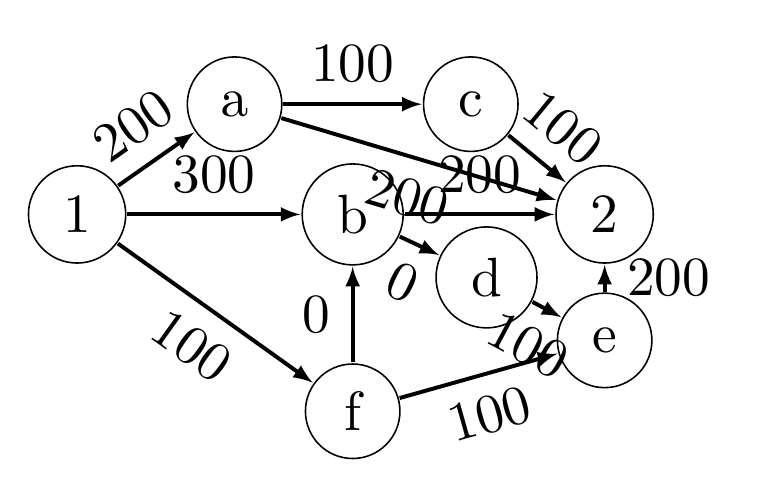
\begin{tikzpicture}[>=latex,shorten >=0.1pt,auto, thick,node distance=2.0cm]
\node (a) [draw , circle, minimum size= 0.5cm, line width=0.2mm] at (0.0,0.3) {1};
\node (b) [draw , circle, minimum size= 0.6cm, line width=0.2mm] at (2.0,1.7) {a};
\node (c) [draw , circle, minimum size= 0.6cm, line width=0.2mm] at (5.0,1.7) {c};
\node (d) [draw , circle, minimum size= 0.5cm, line width=0.2mm] at (3.5,0.3) {b};
\node (e) [draw , circle, minimum size= 0.5cm, line width=0.2mm] at (6.7,0.3) {2};
\node (f) [draw , circle, minimum size= 0.6cm, line width=0.2mm] at (3.5,-2.2) {f};
\node (g) [draw , circle, minimum size= 0.6cm, line width=0.2mm] at (6.7,-1.3) {e};
\node (h) [draw , circle, minimum size= 0.5cm, line width=0.2mm] at (5.2,-0.5) {d};
\path[->,line width=0.5mm]
(a) edge              node [sloped,above] {200} (b)
(b) edge              node {100} (c)
(c) edge              node [above,sloped] {100} (e)
(b) edge              node [below,sloped] {200} (e)
(a) edge              node {300} (d)
(d) edge              node {200} (e)
(d) edge              node [below ,sloped] {0} (h)
(h) edge              node [below,sloped] {100} (g)
(g) edge              node [right]{200} (e)
(a) edge              node [below, sloped] {100} (f)
(f) edge              node [below,sloped] {100} (g)
(f) edge              node [left] {0} (d);
\end{tikzpicture}



%https://gateoverflow.in/204122/gate2018-47
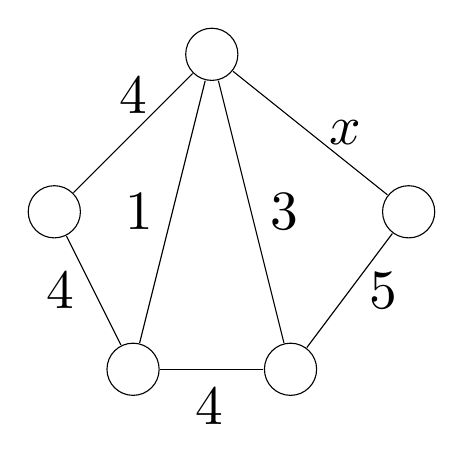
\begin{tikzpicture}
\tikzstyle{every node}=[scale=2,auto]

\node[shape=circle,draw=black] (A) at (-2,0) {};
\node[shape=circle,draw=black] (B) at (0,2) {};
\node[shape=circle,draw=black] (C) at (2.5,0) {};
\node[shape=circle,draw=black] (D) at (-1,-2) {};
\node[shape=circle,draw=black] (E) at (1,-2) {};
   
\path [-] (A) edge node[above] {$4$} (B);
\path [-] (B) edge node[right] {$x$} (C);
\path [-] (C) edge node[right] {$5$} (E);
\path [-] (E) edge node[right] {$3$} (B);
\path [-] (E) edge node[below left,pos = 0.2] {$4$} (D);
\path [-] (D) edge node[left] {$4$} (A);
\path [-] (D) edge node[left] {$1$} (B);
   
\end{tikzpicture}

%https://gateoverflow.in/205089/gate2018-aptitude-set-4-ga-6?show=205155#a205155
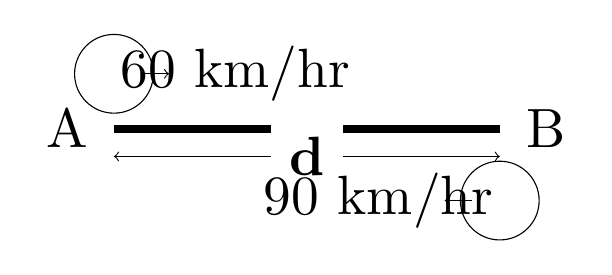
\begin{tikzpicture}[scale=0.7]
\node[,draw,circle,minimum size= 0.5cm] at (-1,0) {} ;
\draw[-,line width = 1mm] (-1,-1) node[left] {A} -- (6,-1)node[right]{B};
\draw[->] (-0.5,0) -- (0,0);
\node[,draw,circle,minimum size= 0.5cm] at (6,-2.3) {} ;
\draw[<-] (5,-2.3) -- (5.5,-2.3);
\path[<->] (-1,-1.5) edge node[ fill=white, anchor=center, pos=0.5,font=\bfseries] {d} (6,-1.5);
%\draw[|<->|](-1,-1.5) -- node[below] {d} (6,-1.5);
\node at (1.2,0){60 km/hr};
\node at (3.8,-2.3) {90 km/hr};
\end{tikzpicture}

%%%%%%%%%%https://gateoverflow.in/313609/gate2018-2-ga-6?show=313610#a313610
  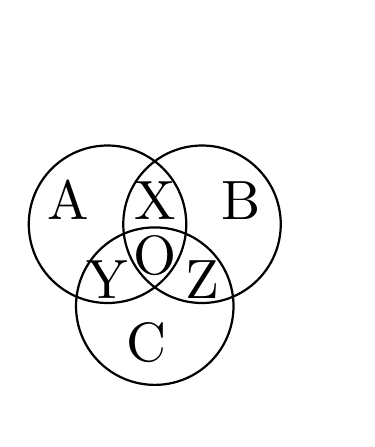
\begin{tikzpicture}[thick]
       
        \draw (0,0) circle (1) node[above,shift={(0,1)}] {${}$};
        \draw (1.2,0) circle (1) node[above,shift={(0,1)}] {${}$};
        \draw (.6,-1.04) circle (1) node[shift={(1.1,-.6)}] {${}$};

        \node at (.6,-.4) {O};
        \node at (1.2,-.7) {Z};
        \node at (0,-.7) {Y};
        \node at (1.7,.3) {B};
        \node at (.6,.3) {X};
        \node at (-0.5,.3) {A};
       
      
        \node at (.5,-1.5) {C};
       
\end{tikzpicture}






